
% This LaTeX was auto-generated from MATLAB code.
% To make changes, update the MATLAB code and republish this document.

\documentclass{article}
\usepackage{graphicx}
\usepackage{color}

\sloppy
\definecolor{lightgray}{gray}{0.5}
\setlength{\parindent}{0pt}

\begin{document}

    
    
\section*{INTRODUCTION TO COMPRESSIVE SENSING}

\begin{par}
This script is an introduction to sparse signal representation and compressive sensing.
\end{par} \vspace{1em}

\subsection*{Contents}

\begin{itemize}
\setlength{\itemsep}{-1ex}
   \item Basis Representation Fundamentals
   \item Example dictionary for 2D-DCT transformation
   \item Uncertainty Principle
   \item Sines and spikes example
   \item Minimum Energy Decomposition - $l_2$ norm
   \item Sparse decomposition
   \item Compressed Sensing
   \item Algorithms for Sparse Recovery
   \item Univariate Thresholding
   \item $l_0$-norm Minimization
   \item $l_1$-norm Minimization
   \item ALGORITHMS FOR $l_0$-norm minimization
\end{itemize}
\begin{verbatim}
close all
clearvars
clc
\end{verbatim}


\subsection*{Basis Representation Fundamentals}

\begin{par}
Every signal $x\in\mathbf{R}^N$ is representable in terms of $N$ coefficients $\{s_i\}_{i=1}^N$ in a given basis $\{\psi_i\}_{i=1}^{N}$ for $\mathbf{R}^N$ as
\end{par} \vspace{1em}
\begin{par}
$$x= \sum\limits_{i=1}^N \psi_i s_i$$
\end{par} \vspace{1em}
\begin{par}
Arranging the $\psi_i$ as columns into the $N\times N$ matrix $\Psi$ and the coefficients $s_i$ into the $N\times 1$ coefficient vector $\textbf{s}$, we can write that $x=\Psi s$, with $s\in\mathbf{R}$.
\end{par} \vspace{1em}
\begin{par}
We say that signal $x$ is $K$-sparse in the basis $\Psi$ if there exists a vector $s\in\mathbf{R}^N$ with only $K\ll N$ nonzero entries such that $x=\Psi s$.
\end{par} \vspace{1em}
\begin{par}
If we use basis matrix containing $N$ unit-norm column vectors of length $L$ where $L<N$ (i.e. $\Psi\in\mathbf{R}^{L\times N}$), then for any vector $x\in\mathbf{R}^L$ there exist infinitely many decompositions $s\in\mathbf{R}^N$ such that $x=\Psi s$. We refer to $\Psi$ as the overcomplete sparsifying dictionary.
\end{par} \vspace{1em}
\begin{par}
Sparsifying dictionary can be:
\end{par} \vspace{1em}
\begin{enumerate}
\setlength{\itemsep}{-1ex}
   \item chosen from a known set of transforms like DCT, wavelet...
   \item learnt from data
\end{enumerate}


\subsection*{Example dictionary for 2D-DCT transformation}

\begin{verbatim}
figure
visualizeDictionary(kron(dctmtx(8),dctmtx(8))')
title('2D-DCT Dictionary')
figure
haar1D = full(wmpdictionary(8, 'lstcpt', {{'haar',3}}));
visualizeDictionary(kron(haar1D, haar1D))
title('2D-DWT Dictionary - HAAR')
\end{verbatim}

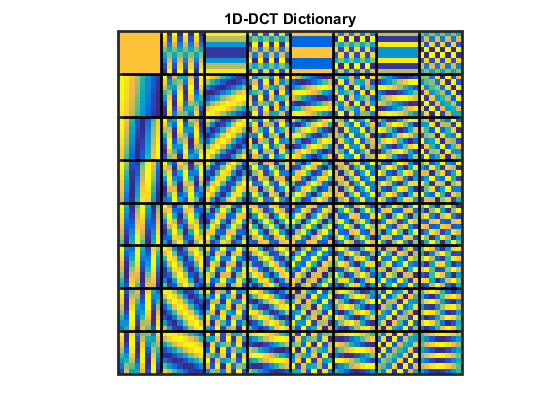
\includegraphics [width=4in]{IntroToCompressiveSensing_01.eps}

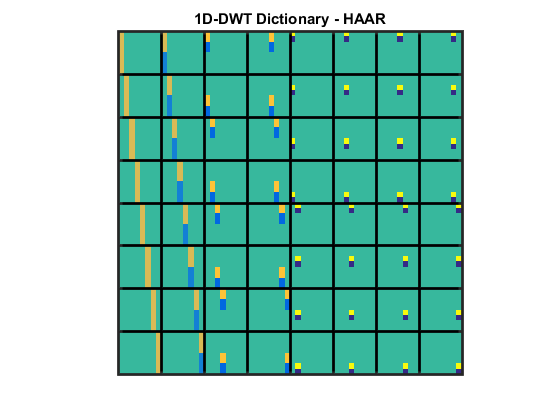
\includegraphics [width=4in]{IntroToCompressiveSensing_02.eps}


\subsection*{Uncertainty Principle}

\begin{par}
As an illustrative example, we will consider the case where our dictionary is the union of two particular orthobases: the identity (spike) basis and the Fourier (sine) basis $\Psi = [I\quad F]$.
\end{par} \vspace{1em}
\begin{par}
Spike and Fourier basis are mutually fully incoherent in the sense that it takes $n$ spikes to build up a single sinusoid and also it takes $n$ sinusoids to build up a single spike.
\end{par} \vspace{1em}
\begin{verbatim}
n = 64;

fourier = (1/sqrt(n))*exp((1j*2*pi*[0:n-1]'*[0:n-1])/n);
spike = eye(n);

psi = [spike, fourier];

% figure
imagesc(real(psi))
axis image
title('Spike/Fourier Dictionary')
\end{verbatim}

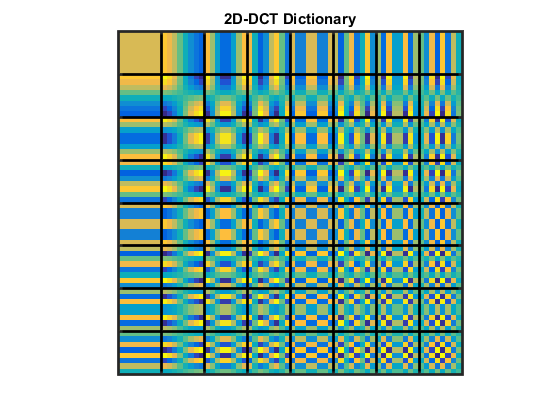
\includegraphics [width=4in]{IntroToCompressiveSensing_03.eps}


\subsection*{Sines and spikes example}

\begin{par}
Now we will create a signal that is a mixture of spikes and sines. As we know that the first half of our matrix $\Psi$ contains spike functions and the second half corresponds to sine functions, we can construct random sparsity pattern with sparsity K and compute $x=\Psi*s$ to obtain a signal which is a mixture of impulses and sinusoids.
\end{par} \vspace{1em}
\begin{verbatim}
%desired sparsity K
K = 2;
%randomly selected basis coefficients
idx = randi([1,2*n], 1, K);

%random sparsity vector
s = zeros(2*n, 1);
s(idx) = 1;

%obtain the signal which is a mixture of impulses and sinusoids
x = psi*s;

%visualize signal
% figure
stem(real(x))
title('Signal - mixture of K impulses and sinusoids')
\end{verbatim}

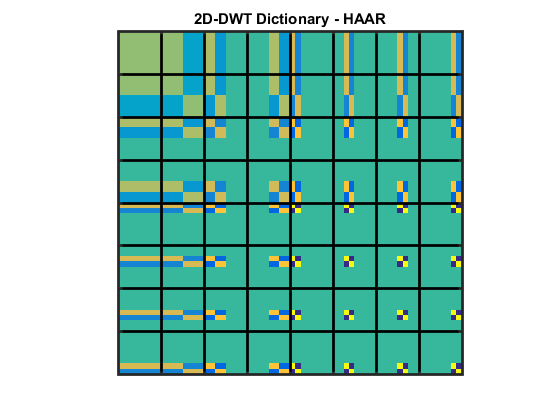
\includegraphics [width=4in]{IntroToCompressiveSensing_04.eps}


\subsection*{Minimum Energy Decomposition - $l_2$ norm}

\begin{par}
There are infinite number of ways we can decompose signal x using atoms from our dictionary. Most natural way would be to use certain basis functions which correspond to previously selected basis function indices. This way we get the sparsest possible representation.
\end{par} \vspace{1em}
\begin{par}
Another way we can get representation for x is by applying $\Psi^*$ and by dividing the result by 2. Since $\Psi\Psi^*=2I$, we get next reproducing formula for x.
\end{par} \vspace{1em}
\begin{par}
$$x=\frac{1}{2}\Psi(\Psi^*x)$$
\end{par} \vspace{1em}
\begin{par}
When we apply $s=\frac{1}{2}\Psi^*x$ we get result that corresponds to the minimum energy decomposition of our signal into a coefficient vector that represents x. Minimum energy solution corresponds to $l_2$ norm minimizaton. Unfortunately, minimum energy decomposition almost never yields the sparsest possible soultion. The reason for this is that the vector that a vector has minimum nenergy when its total energy is distribured over all the coefficients of the vector. $l_2$ gives us a solution that is dense, but has small values for the coefficients.
\end{par} \vspace{1em}
\begin{par}
Our ability to separate sines part from the spikes part of our signal of interest is what will determine whether or nor we can find a unique sparse decomposition. Being able to tell these two components apart comes from a new kind of uncertainty principle which states that a signal can't be too sparse in time and frequency domain simoultaneously.
\end{par} \vspace{1em}
\begin{verbatim}
%minimum energy decomposition
s = psi'*x;

% figure
stem(real(s))
title('Minimum energy decomposition - l_2 norm')
\end{verbatim}

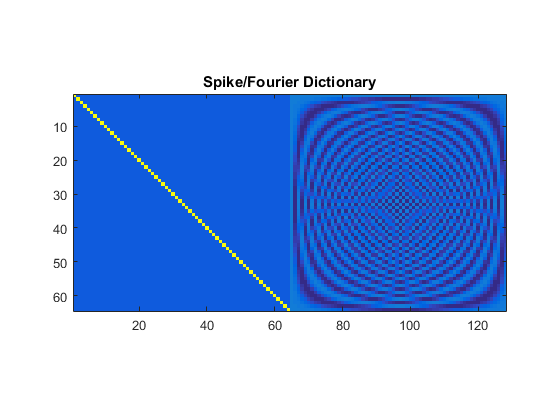
\includegraphics [width=4in]{IntroToCompressiveSensing_05.eps}


\subsection*{Sparse decomposition}

\begin{par}
Since our goal of finding sparsest possible representation of our signal $x$ over some basis $\Psi$ is equivalent to finding the solution with the smallest number of nonzero elements in basis coefficient vector $s$ we will use $l_0$ pseudo-norm to find our solution. Sparse signal recovery can be formulated as finding minimum-cardinality solution to a constrained optimization problem. In the noiseless case, our constraint is simply $x=\Psi s$, while in the noisy case(assuming Gaussian noise), the solution must satisfy $\Vert x-x^*\Vert_2\leq\epsilon$ where $x^*=\Psi s$ is the hypothetical noiseless representation and the actual representation is $\epsilon$-close to it in $l_2$ norm. The objective function is the cardinality of s(number of nonzeros) which is often denoted $\Vert x\Vert_0$ and called $l_0$ norm of $s$.
\end{par} \vspace{1em}
\begin{par}
Optimization problems corresponding to noiseless and noisy sparse signal recovery can be written as:
\end{par} \vspace{1em}
\begin{itemize}
\setlength{\itemsep}{-1ex}
   \item $\min\limits_x\Vert x\Vert_0 \quad s.t. \quad x=\Psi s$
   \item $\min\limits_x\Vert x\Vert_0 \quad s.t. \quad \Vert x-\Psi s\Vert_2\leq\epsilon$
\end{itemize}
\begin{par}
In general, finding a minimum-cardinality solution satisfying linear constraints is an NP-combinatorial problem and an approximation is necessary to achieve computational efficiency. Two main approximation approaches are typically used in sparse recovery: the first one is to address the original NP-combinatorial problem via approximate methods, such as greedy search, while the second one is to replace the intractable problem with its convex relaxation that is easy to solve. In other words, one can either solve the exact problem approximately, or solve an approximate problem exactly.
\end{par} \vspace{1em}
\begin{par}
In figure below, we can see sparse decomposition of our signal of interest. Notice that there are only K coefficients active, while others are equal to zero and that is exactly what we wanted to achieve.
\end{par} \vspace{1em}
\begin{verbatim}
%sparse decomposition
nIter = 10;
s = sparseCode(x, psi, K, nIter);

% figure
stem(real(s))
title('Sparse decomposition - l_0 norm')
\end{verbatim}

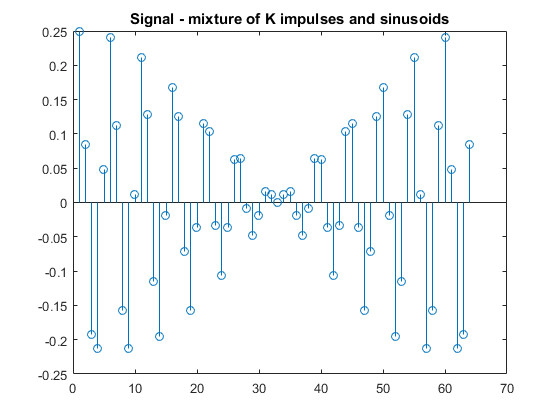
\includegraphics [width=4in]{IntroToCompressiveSensing_06.eps}


\subsection*{Compressed Sensing}

\begin{par}
The key idea behind compressive sensing is that the majority of real-life signals(images, audio...) can be well approximated by sparse representation vectors, given some appropriate basis $\Psi$, and that exploiting the sparse signal structure can dramatically reduce the signal acquisition cost. Traditional approach to signal acquisition is based on the classical Shannon- Nyquist result stating that in order to preserve information about a signal, one must sample the signal at a rate which is at least twice the signal's bandwidth, defined as the highest frequency in the signal's spectrum. Note, however, that such classical scenario gives a worst-case bound, since it does not take advantage of any specific structure that the signal may possess. In practice, sampling at the Nyquist rate usually produces a tremendous number of samples, e.g., in digital and video cameras, and must be followed by a compression step in order to store or transmit this information efficiently.
\end{par} \vspace{1em}
\begin{par}
The compression step uses some basis to represent a signal (e.g., Fourier, wavelets, etc.) and essentially throws away a large fraction of coefficients, leaving a relatively few important ones. Thus, a natural question is whether the compression step can be combined with the acquisition step, in order to avoid the collection of an unnecessarily large number of samples.
\end{par} \vspace{1em}
\begin{par}
Compressive sensing offers positive answer to the above question. Let $x\in\mathbf{R}^N$ be a signal that can be represented sparsely in some basis $\Psi$ i.e. $x=\Psi s$ where $\Psi$ is an $N\times N$ matrix of basis vectors(columns), and where $s\in\mathbf{R}^N$ is a sparse vector of the signal's coordinates with only $K\ll N$ nonzeros. Though the signal is not observed directly, we can obtain a set of linear measurements:
\end{par} \vspace{1em}
\begin{par}
$$y=\Phi x=\Phi\Psi s=A s$$
\end{par} \vspace{1em}
\begin{par}
where $\Psi$ is an $N\times M$ measurement matrix and $y\in\mathbf{R}^M$ is a set of $M$ measurements or samples where $M$ can be much smaller than the original dimensionality of the signal, hence the name compressive sensing(CS).
\end{par} \vspace{1em}
\begin{par}
The central problem of compressed sensing is reconstruction of a high-dimensional sparse signal representation $x$ from a low-dimensional linear observation $y$.
\end{par} \vspace{1em}
\begin{par}

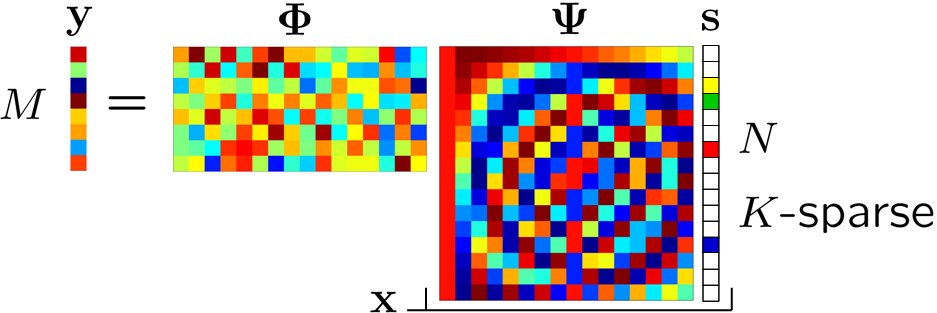
\includegraphics [width=4in]{cs_matrix_form.png}

\end{par} \vspace{1em}
\begin{par}
In general, $l_q$ norms for particular values of $q$, denoted $\Vert x\Vert_q$ or more precisely their $q$-th power $\Vert x\Vert_q^q$ are frequently used as regularizers $R(x)$ in constrained optimization problems:
\end{par} \vspace{1em}
\begin{par}
$$\min\limits_{x\in\mathbf{R}^N} R(x)\quad s.t.\quad y=Ax$$
\end{par} \vspace{1em}
\begin{par}
For a $q\ge 1$, the $l_q$ norm, also called just $q$-norm of a vector $x\in\mathbf{R}^N$ is defined as:
\end{par} \vspace{1em}
\begin{par}
$$\Vert x\Vert_q=(\sum\limits_{i=1}^N\vert x_i\vert^q)^\frac{1}{q}$$
\end{par} \vspace{1em}
\begin{par}
We can now observe relation between cardinality and $\Vert l_q\Vert$-norms. The function $\Vert x\Vert_0$ referred to as $l_0$-norm of $x$ is defined as a limit of $\Vert x\Vert_q^q$ when $q\to0$:
\end{par} \vspace{1em}
\begin{par}
$$\Vert x\Vert_0=\lim\limits_{q\to 0}\Vert x\Vert_q^q=\lim\limits_{q\to 0}\sum\limits_{i=1}^p\vert x_i\vert^q=\sum\limits_{i=1}^p\lim\limits_{q\to 0}\vert x_i\vert^q$$
\end{par} \vspace{1em}
\begin{par}
For each $x_i$, when $q\to 0$, $\vert x_i\vert^q\to I(x_i)$, the indicator function, which is 0 at $x=0$ and 1 otherwise. Thus, $\Vert x\Vert_0=\sum\limits{i=1}^p I(x_i)$, which gives exactly the number of nonzero elements of vector x called cardinality. Using the cardinality function, we can now write the problem of sparse signal recovery from noiseless linear measurements as:
\end{par} \vspace{1em}
\begin{par}
$$\min\limits_x\Vert x\Vert_0 \quad s.t. \quad y=A x$$
\end{par} \vspace{1em}
\begin{par}
As already mentioned before, the above optimization problem is NP-hard and no known algorithm can solve it efficiently in polynomial time. Therefore, approximations are necessary and were already presented before. Under appropriate conditions the optimal solution can be recovered efficiently by certain appproximate techniques.
\end{par} \vspace{1em}
\begin{par}
First approach to approximation is a heuristic-based search such as gready search. In gready search method, one can start with a zero vector and keep adding nonzero coefficients one by one, selecting at each step the coefficient that leads to the best improvement in the objective function(gready coordinate descent). In general, such heuristic search methods are not guaranteed to find the global optimum. However, in practive, they are simple to implement, very computationally efficient and under certain conditions they are even guaranteed to recovel the optimal solution.
\end{par} \vspace{1em}
\begin{par}
An alternative approximation technique is the relaxation approach based on replacing an intractable objective function or constraint by a tractable one. For example, convex relaxations approximates a non-convex optimization problem by a convex one, i.e. by a problem with convex objective and convex constraints. Such problems are known to be "easy", i.e. there  exists a variety of efficient optimization methods for solving convex problems. Clearly, besides being easy to solve, e.g., convex, the relaxed version of the optimization problem must also enforce solution sparsity. In the following sections, we discuss lq-norm based relaxations, and show that the Zi-norm occupies a unique position among them, combining convexity with sparsity. A convex optimization problem is minimization of a convex function over a convex set of feasible solutions defined by the constraints. Convex problems are easier to solve than general optimization problems because of the important property that any local minima of a convex function is also a global one. Optimization problem using $l_1$ norm writes:
\end{par} \vspace{1em}
\begin{par}
$$\min\limits_x\Vert x\Vert_1 \quad s.t. \quad y=A x$$
\end{par} \vspace{1em}


\subsection*{Algorithms for Sparse Recovery}

\begin{par}
We will focus on the noisy sparse recovery problems:
\end{par} \vspace{1em}
\begin{itemize}
\setlength{\itemsep}{-1ex}
   \item $l_0$-norm minimization: $\min\limits_x\Vert x\Vert_0 \quad s.t. \quad \Vert x-\Psi s\Vert_2\leq\epsilon$
   \item $l_1$-norm relaxation:   $\min\limits_x\Vert x\Vert_1 \quad s.t. \quad \Vert x-\Psi s\Vert_2\leq\epsilon$
   \item Lagrangian form $l_1$ minimization (LASSO): $\min\limits_{x}\frac{1}{2}\Vert y-Ax\Vert_2^2+\lambda\Vert x\Vert_1$
\end{itemize}
\begin{par}
Recall that x is an N-dimensional unknown sparse signal, which in a statistical setting corresponds to a vector of coefficients of a linear regression model, where each coefficient $x_i$ signifies the amount of influence the $i$-th input, or predictor variable $A_i$, has on the output $y$, an $M$-dimensional vector of observations of a target variable $Y$. $A$ is an $M\times N$ design matrix, where the $i$-th column is an $M$-dimensional sample of a random variable $A_i$, i.e. a set of $M$ independent and identically distributed, or i.i.d., observations.
\end{par} \vspace{1em}
\begin{par}
We would like to focus on the specific case of orthogonal design matrices. It turns out that in such case both $l_0$- and $l_1$-norm optimization problems decompose into independent univariate problems, and their optimal solutions can be easily found by very simple univariate thresholding procedures.
\end{par} \vspace{1em}


\subsection*{Univariate Thresholding}

\begin{par}
An orthonormal(orthogonal) matrix $A$ is an $N\times N$ square matrix satisfying $A^TA=AA^T=I$ where $I$ denotes the identity matrix. A linear transformation defined by an orthogonal matrix $A$ has a nice property, it preserves the $l_2$-norm of a vector.
\end{par} \vspace{1em}
\begin{par}
$$\Vert Ax\Vert_2^2=(Ax)^T (Ax) = x^T (A^TA) x = x^T x =\Vert x\Vert_2^2$$
\end{par} \vspace{1em}
\begin{par}
The same is also true for $A^T$ and we get:
\end{par} \vspace{1em}
\begin{par}
$$\Vert y-Ax\Vert_2^2=\Vert A^T(y-Ax)\Vert_2^2=\Vert\hat{x}-x\Vert_2^2=\sum\limits_{i=1}^N(\hat{x}_i-x_i)^2$$
\end{par} \vspace{1em}
\begin{par}
where $\hat{x}=A^Ty$ corresponds to the ordinary least squares(OLS) solution when $A$ is orthogonal, i.e. $\hat{x}=\min\limits_{x}\Vert y-Ax\Vert^2$ This transformation of the sum-squared loss will greatly simplify our optimization problems.
\end{par} \vspace{1em}


\subsection*{$l_0$-norm Minimization}

\begin{par}
The problem of $l_0$-norm minimization can now be rewritten as:
\end{par} \vspace{1em}
\begin{par}
$$\min\limits_x\Vert x\Vert_0 \quad s.t. \quad \sum\limits_{i=1}^N(\hat{x}_i-x_i)^2\le\epsilon^2$$
\end{par} \vspace{1em}
\begin{par}
In other words, we are looking for the sparsest (i.e., smallest $l_0$-norm) solution $x^*$ that is $\epsilon$-close in $l_2$-sense to the OLS solution $x = A^T y$.
\end{par} \vspace{1em}
\begin{par}
It is easy to construct such solution by choosing k largest (in the absolute value) coordinates of x and by setting the rest of the coordinates to zero, where k is the smallest number of such coordinates needed to get $\epsilon$-close to $\hat{x}$, i.e. to make the solution feasible.
\end{par} \vspace{1em}
\begin{par}
This can also be viewed as an univariate hard thresholding of the OLS solution $\hat{x}$, namely:
\end{par} \vspace{1em}
\begin{par}

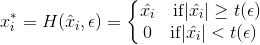
\includegraphics [width=4in]{hard_thresholding.png}

\end{par} \vspace{1em}
\begin{par}
where $t(\epsilon)$ is a threshold value below the $k$-th largest, but above the $(k+1)$-th largest value among $\{\hat{x}_i\}$.
\end{par} \vspace{1em}
\begin{verbatim}
%hard thresholding
hardThresholding = @(x, th) x.*(abs(x)>=th);

x = -1:0.01:1;
threshold = 0.35;
x_ht = hardThresholding(x, threshold);

figure, axis tight
plot(x, x_ht)
hold on
plot([-threshold:0.01:threshold], [-threshold:0.01:threshold], '-.')
title('Hard Thresholding Operator')
xlabel('x')
ylabel('x*')
\end{verbatim}

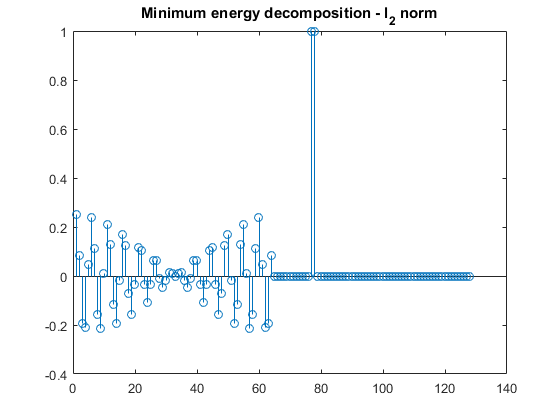
\includegraphics [width=4in]{IntroToCompressiveSensing_07.eps}


\subsection*{$l_1$-norm Minimization}

\begin{par}
For an orthogonal $A$, the LASSO problem becomes:
\end{par} \vspace{1em}
\begin{par}
$$\min\limits_{x}\frac{1}{2}\sum\limits_{i=1}^N(\hat{x}_i-x_i)^2+\lambda \sum\limits_{i=1}^N\vert x_i\vert$$
\end{par} \vspace{1em}
\begin{par}
which trivially decomposes into $N$ independent, univariate optimization problems, one per each $x_i$ variable, $i=1,...N$:
\end{par} \vspace{1em}
\begin{par}
$$\min\limits_{x_i}\frac{1}{2}(\hat{x}_i-x_i)^2+\lambda\vert x_i\vert$$
\end{par} \vspace{1em}
\begin{par}
Global minimum solution for $l_1$-norm minimization can be obtained using soft thresholding operator:
\end{par} \vspace{1em}
\begin{par}
$$x_i^*=S(\hat{x},\lambda)=sign(\hat{x}(\vert \hat{x}\vert)-\lambda)_+$$
\end{par} \vspace{1em}
\begin{par}
When the design matrix $A$ is orthogonal, both $l_0$- and $l_1$-norm minimization problems decompose into a set of independent univariate problems which can be easily solved by first computing the OLS solution $\hat{x}=A^Ty$ and then applying thresholding operators to each coefficient.
\end{par} \vspace{1em}
\begin{verbatim}
%soft thresholding
softThresholding = @(x, th) sign(x).*max(abs(x)-th,0);

x = -1:0.01:1;
threshold = 0.35;
x_st = softThresholding(x, threshold);

figure, axis tight
plot(x, x_st)
hold on
plot(x, x, '-.')
title('Soft Thresholding Operator')
xlabel('x')
ylabel('x*')
\end{verbatim}

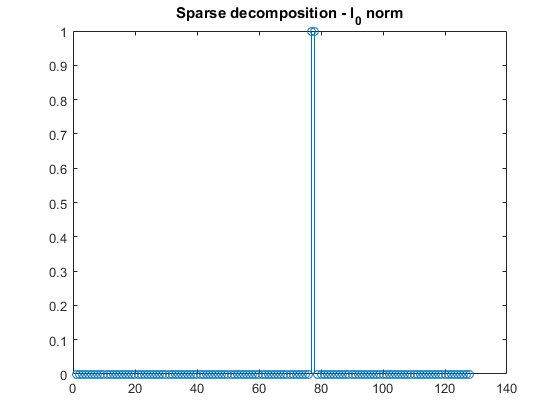
\includegraphics [width=4in]{IntroToCompressiveSensing_08.eps}


\subsection*{ALGORITHMS FOR $l_0$-norm minimization}

\begin{par}
In this section we focus on approximate optimization methods such as greedy approaches for solving $l_0$-norm minimization problems:
\end{par} \vspace{1em}
\begin{par}
$$\min\limits_x\Vert x\Vert_0 \quad s.t.\quad \Vert y-Ax\Vert_2\leq\epsilon$$
$$\min\limits_x\Vert y-Ax\Vert_2 \quad s.t.\quad \Vert x\Vert_0\leq\k$$
\end{par} \vspace{1em}
\begin{par}
In the second form of the optimization problem $k$ represents bound on the number of nonzero elements and is uniquely defined by parameter $\epsilon$ in the first formulation of the problem. The latter problem is also known as the best subset selection problem, since it aims at finding a subset of $k$ variables that yield the lowest quadratic loss, i.e. the best linear regression fit.
\end{par} \vspace{1em}
\begin{par}
At high-level greedy algorithmic scheme can be outlined as: \# Start with an empty support set, i.e. the set of nonzero variables , and zero vector as the current solution \# Select the best variable using some ranking cirterion $C_{rank}$, and add the variable to the current support set. \# Update the current solution, and recompute the current objective function, also called the residual. \# If the current solution $x$ satisfies a given stopping criterion $C_{stop}$, exit and return $x$, otherwise go to step 2.
\end{par} \vspace{1em}



\end{document}
    
